\begin{problem}{}{input.csv}{output.csv}{2 секунды}{256 мегабайт}
% Pandas: Data Cleaning

Під час роботи з даними часто виникає потреба в їх очищенні, оскільки вони можуть містити різні недоліки, 
такі як пропущені значення, дублікати, невірні типи даних або навіть непотрібні пробіли.
Бібліотека Pandas відкриває широкі можливості для очищення даних.

Є таблиця даних. Таблиця зберігається у форматі СSV (Character-Separated Values), поля відокремлюються символом \texttt{<<;>>}.
Кожна комірка цієї таблиці може бути:
\begin{itemize}[topsep=0pt,itemsep=0pt,parsep=0pt,partopsep=0pt]
  \item[-] цілим числом;
  \item[-] дробовим числом;
  \item[-] пустою;
  \item[-] заповнена пробільними символами (пробілами або табуляціями);
  \item[-] символьним рядком.
\end{itemize}

\begin{center}
  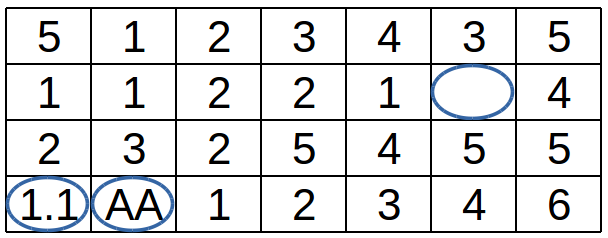
\includegraphics[width=0.40\textwidth]{pic1.png}
\end{center}

Вам треба виконати очистку цих даних:
\begin{enumerate}
  \item Спочатку видалити всі рядки, в яких не всі значення є цілими числами.
  \item Потім видалити всі стовпчики, в яких середне арифметичне всіх значень дорівнює середньому геометричному.
\end{enumerate}

\begin{center}
  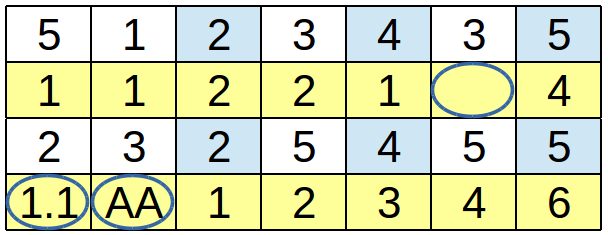
\includegraphics[width=0.40\textwidth]{pic2.png}
\end{center}

\InputFile
Вашій програмі на вхід подається файл \texttt{input.csv}, який містить вказану таблицю з данними.
Кількість рядків та кількість стовпчиків в таблиці не перевищують $1\,000$.

\OutputFile
У файл \texttt{output.csv} запишіть очищену таблицю, поля таблиці відокремлюйте символом \texttt{<<;>>}.

Якщо для очищення даних треба видалити всю таблицю, то в файл \texttt{output.csv} виведіть повідомлення:  \texttt{<<Empty DataFrame>>}.

\Example
\begin{example}
\exmpfile{input.csv}{output.csv}%
\end{example}


\end{problem}

